\section{Prior Work}

Work on Reagent principally concerns bringing together two discrete lines
of work. The first is prior work on building intelligent system that are
capable of combining multimodal input to generate an intent for the user.
Historically, these systems have fallen into the category of ``smart rooms''
where multimodal input is much more of a necessity for more ``natural''
interaction than traditional desktop environments. In these multimodal
``smart rooms'', various efforts have been shown for picking up
where a user is pointing and using it in combination with
their voice to generate a command
\cite{bolt_put-that-there:_1980,carbini_wizard_2006,langner_multiple_2019,farrell_symbiotic_2016,kephart_embodied_2019}.
However, these systems hand-build their display layer and
content to embed the necessary instrumentation for combining speech
and gesture. Alternatively, \cite{coen_sodabot:_1994,brooks_intelligent_1997} demonstrate a system that
hooks into the X display server and could act on the content that was passed through
it from various applications, such as Netscape. While a very powerful approach, it
does not easily work across platforms, and that the security model of modern
applications such as Chrome renders the approach
increasingly impossible. Perhaps the most radical, \cite{roman_middleware_2002} propose an entire middleware infrastructure, similar to an OS,
to underpin these multimodal applications, but this approach
even more readily runs into the aforementioned bottleneck
in that all applications must be built from the ground up to 
utilize this middleware, rendering it hard to reuse existing
content and displays.

Secondly, we look at the rich research on automatic extraction of
information from webpages and the lessons learned there, especially in how
they might work with ontology 
building. \cite{cimiano_towards_2004,hutchison_ontology_2005} propose frameworks on parsing
important information from web pages, which would be then encoded into RDF structures.
\cite{hutchison_comparison_2013} provides a recent
overview of available technologies in this space.
However, these approaches generally focus on the use of just natural language understanding over
the entire page for key terms and relations, and not necessarily leveraging the increasingly
rich ways the data may be shown in a page that require true DOM traversal and analysis. However,
in analysis and automatic parsing of the DOM structure, we are informed by prior work on taking
into account elements that are ``noise'' (e.g. ads and popups) which might look well-structured,
but that the user most likely does not care about. \cite{gupta_dom-based_2003}
utilizes the full DOM-tree to determine relevance of elements. \cite{joshi_web_2009} utilizes both
DOM traversal and NLP to determine salient details. \cite{sun_dom_2011} utilize a algorithm that considers
content density within nodes. Our current work focuses on automatic analysis of elements that
rarely, if ever, appear within this ``noisy'' data, but is important to consider as we expand Reagent to further domains. Finally, in the realm of understanding purely
tabular data, \cite{hackinger_datagorri:_2018} proposes a system similar in some regards to
\textit{Reagent}, but that it requires for any new site the human to first identify the table on the
page and to present a ``template'' on how it should be parsed, acting far less autonomously than
\textit{Reagent}. These works inform our approach
on building \textit{Reagent}, but it is important to note that our end-goal, principally in
automatic on-the-fly webpage parsing and ontology building for use in multimodal applications, is different.

\begin{figure}
    \centering
    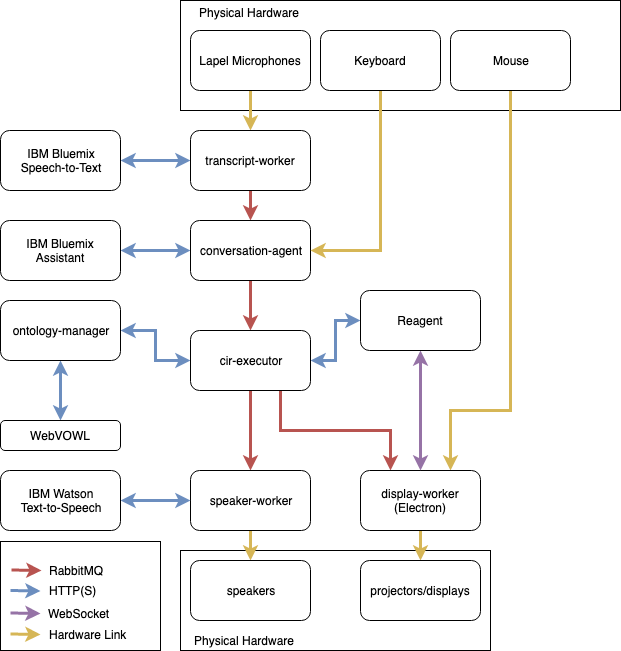
\includegraphics[width=0.45\textwidth]{chapters/03_reagent/figures/cir_diagram}
    \caption{Diagram of the Cognitive and Immersive System for Reagent}
    \label{fig:cais}
\end{figure}